%!TEX TS-program = xelatex
%!TEX encoding = UTF-8 Unicode
%!TeX spellcheck = it_IT
%!TEX root = ../tesi.tex

\chapter{Modello a ostacoli}\label{chap:modello-a-ostacoli}
%
\section{Modelli di radiopropagazione}\label{sec:modelli-propagazione}
Un modello di radiopropagazione (MRP) simula gli effetti dell'attenuazione del segnale radio (segnali elettromagnetici nello spazio libero o etere, in contrasto con la propagazione guidata)
dovuta alla distanza, cammini multipli per effetto della riflessione, ombreggiatura causata dalla presenza di ostacoli.
L'utilizzo di un'idonea rappresentazione per questo tipo di ostacoli è, quindi, necessaria nel contesto di simulazioni di reti VANET in ambienti urbani
e suburbani.
Nel corso degli anni, diversi MRP sono stati proposti.
Il più semplice di questi si chiama modello a disco unitario (\textit{unit-disk model}), nel quale i veicoli possono comunicare fra loro se si trovano entro una certa soglia
di distanza, mentre non possono altrimenti~\cite{6554832}.
Un modello molto utilizzato nelle simuazioni di VANET è il modello a doppio raggio (\textit{Two-ray ground-reflection model}),
nel quale il segnale in fase di ricezione è composto da una componente in linea diretta e una seconda derivante dalla riflessione causata dal terreno~\cite{DBLP:books/daglib/0091821}.
In~\cite{Schmitz:2006:ERW:1164717.1164730} e in~\cite{Souley2005RealisticUS}, modelli più sviluppati prendono in considerazione anche le proprietà riflettenti delle superfici e degli ostacoli.

Tuttavia, un approcio diretto di questo tipo difficilmente scala al numero di nodi necessario in un classico scenario VANET e per questo motivo
spesso tali modelli si affidano a una fase di pre-elaborazione che può richiedere tempi elevati~\cite{Stepanov:2008:IMR:1293378.1293656}.
Per ovviare a questo problema, alcune proposte astraggono dalle informazioni sui singoli edifici, modellando l'ambiente urbano in modo omogeneo
così da creare un modello analitico per l'ombreggiatura~\cite{1492678}.
Questo tipo di modelli riducono il costo computazionale e generalmente si raffrontano bene con i risultati reali;
ciò nonostante, non riescono a catturare effetti a livello mesoscopico come eventuali spazi fra edifici che permetterebbero trasmissioni a corto raggio~\cite{Giordano:2010:CST:1860058.1860065}.

Sono affetti dallo stesso problema anche i modelli (puramente) probabilistici, in quanto non tengono in considerazione la geometria urbana sottostante.
Questi modellano l'effetto dell'ombraggiatura tramite distribuzione stocastiche, fra cui Rice, Rayleigh, Nakagami-m, lognormale e Weibull~\cite{6554832}~\cite{Rappaport:2001:WCP:559977}.
%
\section{Modellazione di ostacoli}\label{sec:modellazione-ostacoli}
Nelle simulazioni di alcuni scenari, come possono essere le VANET, un'accurata rappresentazione della topologia dell'ambiente è necessaria
in quanto limita non solo la mobilità dei veicoli ma interferisce anche con le trasmissioni radio~\cite{7543980}~\cite{amjad2015impact}.
L'attenuazione radio viene spesso modellata in modo deterministico basandosi principalmente sulla distanza della visuale (\textit{Line Of Sight}, LOS)
fra i veicoli, combinando eventualmente un modelli stocastico per considerare l'ombreggiatura.

Negli ultimi anni, diversi studi hanno cercato di rappresentare meglio l'effetto ombreggiatura causato dagli edifici.
In~\cite{Giordano:2010:CST:1860058.1860065} gli autori utilizzavano tecniche di geocodifica inversa (\textit{reverse geocoding}) per estrapolare
informazioni sulla topologia della rete stradale in stile Manhattan. Da qui veniva derivata la geometria degli edifici utilizzata
per differenziare i casi in cui i due veicoli comunicanti avessero la visuale libera (LOS) o meno (\textit{Non Line Of Sight}, NLOS)
e calcolare di conseguenza la potenza del segnale in ricezione.
La configurazione a griglia non è tuttavia applicabile in ogni scenario urbano, speciamente in città italiane storiche,
dove la reste stradale è molto irregolare.
In~\cite{4020783}, invece, le informazioni sugli edifici erano codificate direttamente all'interno dell'ambiente sviluppato, chiamato
EGRESS (\textit{Enviroment for Generating REalistic Scenarios for Simulations}), e permettavano di definire tre tipologie di edifici e altrettanti
percorsi per simulare la mobilità dei nodi; il modello permetteva anche di configurare, con alcuni limiti, diversi tipi di materiale dei pavimenti e dei muri degli edifici.
Questa categorizzazione non permetteva però una buona scalabilità, se si considera che in pochi kilometri quadrati di una città media
ci sono miglialia di edifici.
Gli autori di~\cite{Carpenter:2015:OMI:2756509.2756512} integravano nel noto simulatore di reti Network Simulator 3 (ns-3)~\cite{ns3Website}
un modello a ostacoli empirico precedentemente sviluppato~\cite{5720204} ed
estraevano le informazioni per la geometria degli edifici da una piattaforma gratuita
chiamata OpenStreetMap (OSM)~\cite{osmWebsite}; queste venivano successivamente elaborate da un software per la simuazione della mobilità di veicoli
e utilizzate nel simulatore, differenziando i dati sugli edifici e quelli sulla mobilità dei veicoli;
il modello di propagazione teneva conto della distanza percorsa dal segnale internamente all'ostacolo e del numero di muri esterni che questo attraversava.
La semplicità computazionale, l'assenza di pre-elaborazioni, la possibilità di integrare informazioni reali sull'ambiente
e l'integrazione con ns-3 erano alcuni dei punti a favore di questo modello.
%
\section{Il modello matematico}\label{sec:il-modello-matematico}{\vspace*{-.3\baselineskip}} % fix: dunno why so a large space
Il modello a ostacoli utilizzato viene descritto per la prima volta in~\cite{5720204}, dove viene presentato
come un'estensione dei cosiddétti modelli di attenuazione del segnale.
In generale, questi possono essere scritti nella forma dell'Equazione~\ref{eq:fading-models}, dove $P$ è la potenza del trasmettitore (e ricevitore),
$G$ i guadagni delle antenne e $L$ il termine che indica le attenuazioni dovute alla trasmissione.
%
\begin{gather}
	P_r[dBm] = P_t[dBm] + G_t[dB] + G_r[dB] - \sum L_x[dB] 														\label{eq:fading-models} \\
	L_{TwoRayGround} = 10 \lg \left( \frac{d^4 L}{h^2_t h^2_t} \right)	\qquad [dB]		\label{eq:tworayground-model} \\
	L_{LogNorm} = 10 \lg \left( X_\sigma \right)	\qquad [dB]													\label{eq:lognorm-model}
\end{gather}
%
Questi modelli possono essere espressi come componenti di $L$ e concatenati in modo da ottenere l'attenuazione totale risultante.
Ad esempio, le equazioni~\ref{eq:tworayground-model} e~\ref{eq:lognorm-model} illustrano rispettivamente i modelli a doppio raggio e log-normale.
Il modello in esame rappresenta la perdita di segnale dovuta a un ostacolo estendendo l'Equazione~\ref{eq:fading-models}
col termine $L_{s,o}$, che unisce l'attenuazione causata dai bordi dell'ostacolo (attenuazione per-parete)
e quella derivante dalla superficie interna (attenuazione per-metro):
%
\begin{gather}\label{eq:osbtacle-model}
	L_{s,o} = \alpha n + \beta d_o
\end{gather}
dove $n$ è il numero di volte che il bordo dell'ostacolo viene intersecato dalla visuale e $d_o$ è la distanza, in metri, attraversata all'interno dell'ostacolo.
Il primo dei due parametri di calibrazione, $\alpha$, espresso in decibel per metro (dB/m), descrive l'attenuazione
che la trasmissione subisce a causa delle pareti esterne dell'ostacolo.
Il secondo, $\beta$, espresso in decibel (dB per parete), serve come misura di approssimazione della struttura interna dell'ostacolo.
Tramite la regolazione di questo valore è possibile rappresentare diverse tipologie di ostacoli.
Prendendo il caso di edifici in un ambiente cittadino, i valori predefiniti per i due parametri sono $\alpha = 9$ dB per parete e $\beta = 0,4$ dB/m.
Nell'esempio raffigurato in \figurename~\ref{fig:scenario-urbano-1} la visuale fra i due veicoli interseca $n=6$ muri e una distanza interna di $d_o=32$m
e se si sostiuiscono i valori in~\ref{eq:osbtacle-model} si ottiene: $L_{s,o} = 9*6 + 0,4*32 = 66,8$dB.
Solo considerando questa attenuazione la potenza del segnale si riduce di molto, considerando che,
a titolo esemplificativo, nello standard $802.11$b a $11$ Mb/s il limite per la ricezione è di $-89$ dBm;
si evince come, in questo caso, sia difficile che la trasmissione da un veicolo
possa essere ricevuta con successo da un secondo veicolo.
%
\begin{figure}[htbp]
	\centering
		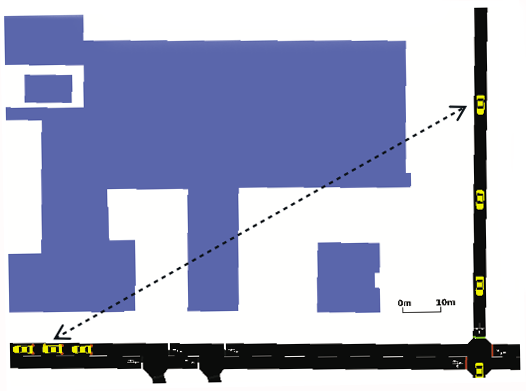
\includegraphics[width=.6\textwidth]{carpenter-1.png}
\caption{Esempio di scenario urbano.\label{fig:scenario-urbano-1}}
\end{figure}
%
%
\section{L'implementazione}\label{sec:implementazione}
Ripredendo il modello ideato in~\cite{5720204} e descritto nella sezione precedente, in~\cite{Carpenter:2015:OMI:2756509.2756512} gli autori ne hanno sviluppato
un'efficiente implementazione per il software di simulazioni ns-3, chiamata semplicemente \textit{Obstacle Shadowing} (ombreggiatura da ostacoli).
Un ostacolo è rappresentato come un poligono bidimensionale, internamente riprodotto da una lista di vertici $(x,y)$, dove questo delimita
il confine (i bordi) dell'ostacolo.
Nella sua implementazione, distrubita come modulo aggiuntivo per il simulatore ns-3,
sono state utilizzate le Computational Geometry Algorithms Library (CGAL), libreria scritta in \Cpp contente algoritmi di geometria computazionale.
Gli ostacoli sono raggruppati in una struttura algebrica dedicata, chiamata partizione binaria dello spazio (\textit{Binary Search Partition}, BSP), utilizzata
per motivi di ottimizzazione.

Nel dettaglio, quando bisogna calcolare l'attenuazione del segnale fra due elementi, nodi in ns-3, si prende in considerazione un riquadro di delimitazione
che include i due e lo si estende
di un certo raggio, ad esempio $200$ metri; i potenziali ostacoli si trovano
selezionando quelli il cui punto centrale risiede all'interno del riquadro, utilizzando il BSP per la ricerca.
Ogni ostacolo selezionado viene controllato per verificare se interseca la visuale
(in questo caso \textit{obstructed-line-of-sight}, OLOS), fra i due nodi.
Se questa verifica ha esito positivo viene cacolato il numero di intersezioni, la distanza interna percorsa e,
successivamente, restituita la quantità di attenuazione secondo la Formula~\ref{eq:osbtacle-model};
questo processo è riassunto nell'Algoritmo~\ref{algo:algoritmo-getobstucteddistancebetween}.
Infine, come ulteriore ottimizzazione, il valore calcolato viene salvato e riutilizzato nel caso i nodi non si siano spostati per più di $0,1$ metri.
%
\begin{italianalgorithm}[h]
\caption{Algoritmo per determinare il numero di intersezioni con i bordi dell'ostacolo e la distanza interna percorsa fra due punti.}\label{algo:algoritmo-getobstucteddistancebetween}
\begin{algorithmic}[1]
	\Procedure{GetObstuctedDistanceBetween}{$p_1, p_2, B$}
	\BState{}\emph{Input}: $p_1, p_2$: posizione dei due veicoli; $B$: partizione binaria dello spazio (BSP) di ostacoli.
	\BState{}\emph{Output}: Distanza interna percorsa $m_o$ e il numero di intersezioni con i bordi $n$.
	\State{$m_o \gets 0;\; n \gets 0$}
	\TextState{Inizializza la portata massima $r$: distanza dal punto $p_1$ o $p_2$ al centro di un ostacolo, utilizzata per filtrare il sottoinsieme di ostacoli sufficientemente vicini.}
	\TextState{Crea un riquadro di delimitazione $b$ per $p_1$ e $p_2$ ed estendila di $r$ in tutte le direzioni.}
	\TextState{Calcola l'insieme di potenziali ostacoli $O$ da quelli all'interno di $b$ in $B$.}
	\ForEach{ostacolo $o \in O$}
		\If{(distanza($p_1$, o.centro) $< r$) $\vee$ (distanza($p_2$, o.centro) $< r$)}
			\ForEach{spigolo $e \in o$}\label{algo:line:getobstucteddistancebetween-interesezione}
				\If{$s$ interseca un raggio da $p_1$ a $p_2$}
					\State{$n \gets n+1$}
					\TextState{Salva la distanza minima e massima da $\{ p_1, p_2\}$ al punto d'intersezione.}
				\EndIf{}
				\TextState{$m_o \gets m_o+$ differenza fra i valori min e max calcolati al passo precedente.}
			\EndFor{}
		\EndIf{}
	\EndFor{}
	\Return{$m_o$ e $n$}
	\EndProcedure{}
\end{algorithmic}
\end{italianalgorithm}
%
Per quanto rigurda la struttura del codice in ns-3, il modello è implementato in tre classi:
\textsf{Obstacle} contiente la rappresentazione geometrica dell'ostacolo come anche i parametri dell'attenuazione per-metro e per-muro.
\textsf{Topology} legge il file contente le informazioni sugli ostacoli (vedere capitolo successivo) e per ognuno di questi
lo crea e lo posiziona all'interno della struttura dati BSP.
La terza, \textsf{ObstacleShadowingPropagationLossModel}, estende ns-3 aggiungendo il modello di propagazione a ostacoli
e richiama \textsf{Topology} nel momento in cui si rende necessario calcolare l'attenuazione del segnale fra due nodi,
utilizzando l'Algoritmo~\ref{algo:algoritmo-getobstucteddistancebetween}.
Il tutto è incluso in un nuovo modulo chiamato \textsf{obstacle} (ostacolo).
%
\section{Estensione a tre dimensioni}\label{sec:estensione-a-tre-dimensioni}
Come detto in precedenza, gli oggetti sono rappresentati da poligoni bidimensionali e, conseguentemente,
il modello descritto lavora in una proiezione bidimensionale dell'ambiente (tridimensionale) di ns-3,
prendendo quindi in considerazione solo le prime due componenti \textit{x} e \textit{y} della posizione di ogni nodo.

Uno dei principali motivi che portò gli ideatori del modello a questa scelta fu la mancanza di sufficienti informazioni tridimensionali
sulla piattaforma dalla quale aquisivano i dati (OpenStreetMap, OSM).
Grazie a una crescente diffusione di Internet sia a livello tecnologico che nella vita quotidiana delle persone,
informazioni di questo tipo sono e saranno sempre più disponibili.
Dato, quindi, il supporto nativo alla terza dimensone di ns-3 (a differenza dei suoi predecessori)
è naturale pensare di estendere il modello affinché
tenga conto di questa componente e pertanto dell'esatta posizione del nodo nell'ambiente tridimensionale.
%
\paragraph{Altezza degli ostacoli}%\label{subsec:altezza-edifici}
Sebbene le forma degli ostacoli si possa descrivere esclusivamente in due dimensioni (punti bidimensionali che ne delineano il perimetro al suolo),
OSM prevede la possibilità di definire l'altezza totale in metri e/o specificare il numero di piani (sopra e sotto il livello del suolo)
nel caso di edifici.
Queste informazioni possono essere sfruttate per creare una forma tridimensionale semplificata dell'ostacolo,
sia che sia presente il vero valore dell'altezza sia che ci siano solo indicati il numero di piani,
anche se in questo caso si tratterebbe solo di una stima e non della dimensione esatta.
%
\begin{figure}[htbp]
	\centering
		\fbox{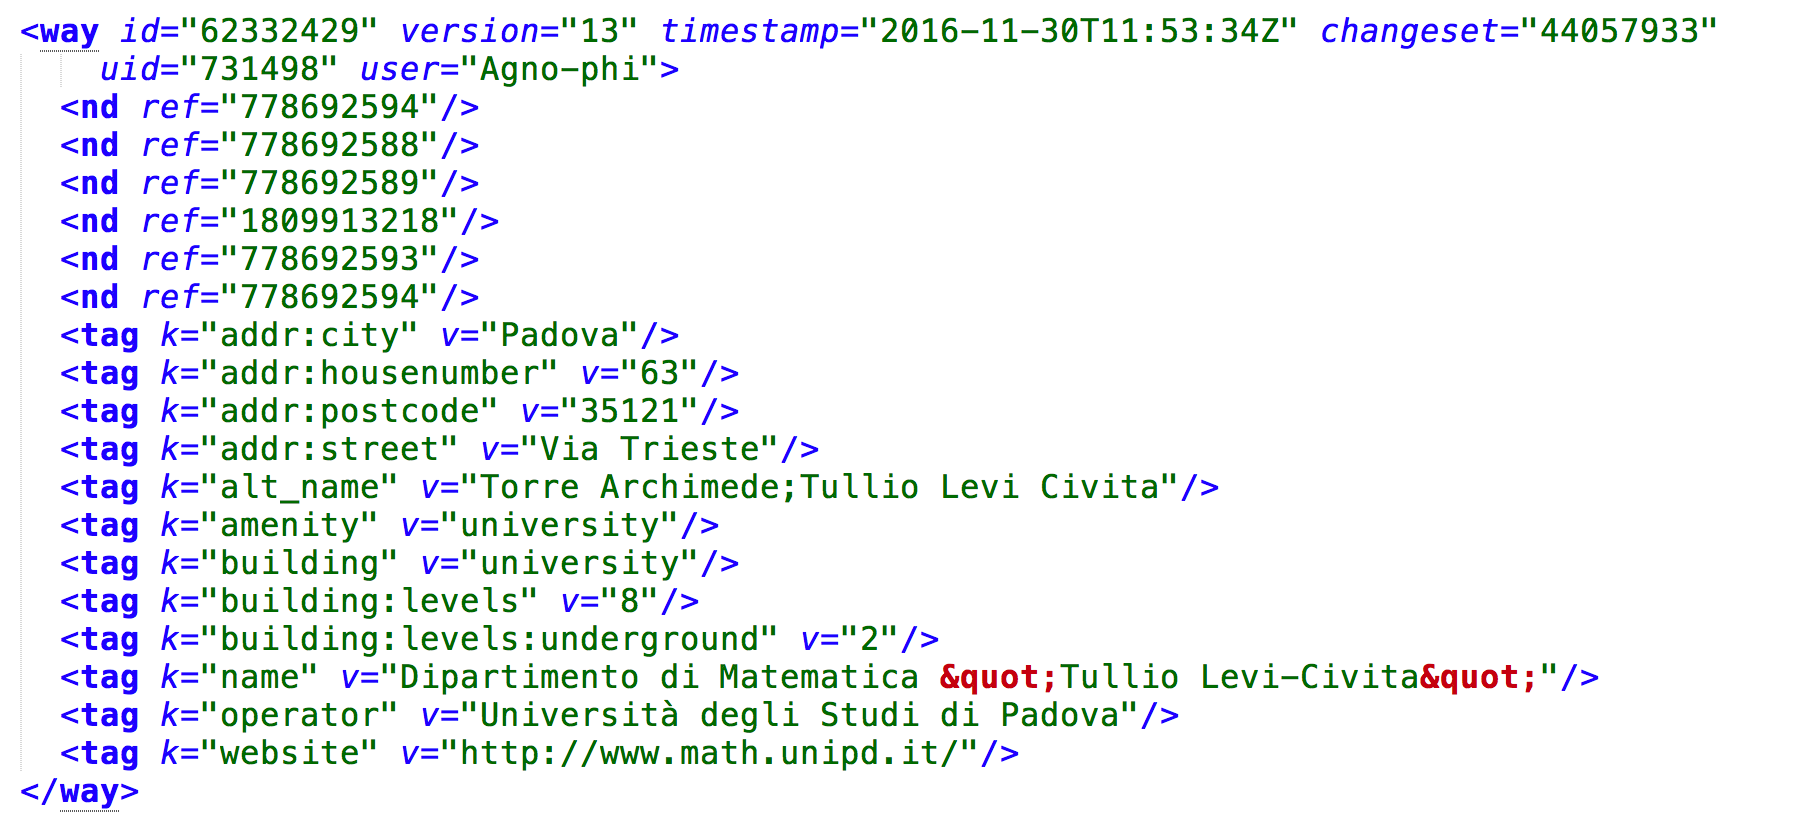
\includegraphics[width=\textwidth]{file-pd-osm-unipd.png}}
\caption{File dati estratto da OSM in cui compaiono informazioni sull'altezza di un edificio.\label{fig:esempio-pd-osm-edificio-altezza}}
\end{figure}
%
Nell'esempio indicato nel \figurename~\ref{fig:esempio-pd-osm-edificio-altezza}, manca la misura dell'altezza ma è presente
il numero di piani: è sufficiente moltiplicare questo numero, qui $8$, per l'altezza media un piano, per esempio $2,7$ metri,
per ottenere una stima dell'altezza pari a $21,6$ metri.
%
\begin{figure}[htbp]
	\centering
	\fbox{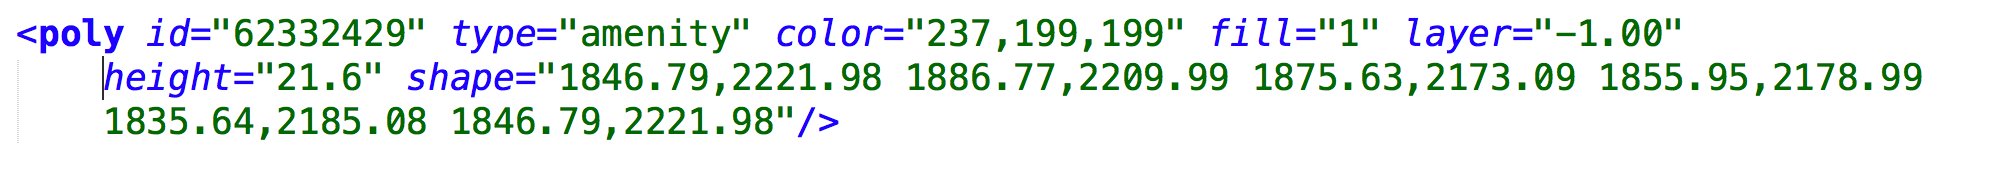
\includegraphics[width=\textwidth]{esempio-poly-blocco-torre.png}}
\caption{Rappresentazione di un edificio in cui è presente un valore di l'altezza.\label{fig:esempio-pd-poly-edificio-altezza}}
\end{figure}
%
A questo punto è necessario decidere la rappresentazione interna dell'ostacolo tridimensionale
e ci sono (almeno) due strade possibili: combinare la forma bidimensionale dell'ostacolo
e l'altezza per creare un poligono tridimensionale (con punti $x,y,z$) oppure
scegliere di tenere le due informazioni separate e gestirle di conseguenza.
Va però fatto notare che si conosce solo forma che questo ha al suolo,
in quanto i punti sono bidimensionali, di conseguenza la forma tridimensionale
sarebbe una proiezione in altezza della stessa.
Mantere separate la forma e l'altezza permette, quindi, di ridurre i costi legati
alla costruzione e alla memorizzazione dell'eventuale poliedro,
senza perdita di informazioni.
%
\paragraph{Modifica all'algoritmo}
Il resto dell'algoritmo \textsf{GetObstuctedDistanceBetween} (Algoritmo~\ref{algo:algoritmo-getobstucteddistancebetween})
rimane sostanzialmente lo stesso e, nello specifico, la ricerca dei potenziali ostacoli rimane invariata.
Infatti gli ostacoli che si interpongono fra due punti nello spazio tridimensionale saranno gli stessi che sul piano bidimensionale
(creato dalla perdita della terza componente \textit{z})
grazie alla forma semplificata dell'oggetto per i motivi esposti precedentemente.
All'oggetto \textsf{Obstacle} è sufficiente aggiungere un campo con il valore dell'altezza.

Le modifiche significative si trovano nel calcolo del numero di intersezioni $n$,
visto che per la distanza $m_o$ basta aggiungere la componente $z$ del punto di intersezione
e il procedimento è lo stesso che nel caso bidimensionale.
In origine, l'intersezione veniva calcolata fra il segmento (raggio) che unisce i due punti e lo spigolo dell'ostacolo considerato in quel
momento, procedura poi iterata per ogni spigolo dell'ostacolo (riga~\ref{algo:line:getobstucteddistancebetween-interesezione}).
Ora bisogna trovare l'intersezione fra il raggio (segmento) e la parete dello spigolo corrente.
Una soluzione soluzione consiste nel generare un piano in corrispondenza della parete,
calcolare l'intersezione fra questo e il segmento e verificare, nel caso ci sia,
che il punto trovato appartenga alla parete dell'oggetto e che non sia esterno.
Per generare il piano a partire dal segmento dello spigolo basta prendere i due vertici dello spigolo
e un terzo vertice generato da uno dei due (a piacere) a cui si imposta la componente $z$ diversa da $0$.
Per chiarire il concetto, si pensi a un semplice edificio: definita la forma alla base (al suolo) i muri sono perpendicolari
al terreno e, a una certa altezza, si trova il tetto con la stessa forma della base;
il punto d'intersezione che interessa si trova sulla faccia del muro corrente.
L'ultimo passo, non necessario nel caso bidimensionale, consiste nel controllare se il raggio (fra i nodi)
interseca la faccia superiore dell'oggetto (il tetto in un edificio), seguendo un procedimento simile
ai casi delle pareti.
Le modifiche sono riportate nell'Algoritmo~\ref{algo:algoritmo-getobstucteddistancebetween-modificato}.
%
\begin{italianalgorithm}[!h]
\caption{Modifica all'algoritmo per includere la terza dimensione.}\label{algo:algoritmo-getobstucteddistancebetween-modificato}
\begin{algorithmic}[1]
	\Procedure{GetObstuctedDistanceBetween}{$p_1, p_2, B$}
	\State{\ldots}
	\setcounter{ALG@line}{7}
	\ForEach{ostacolo $o \in O$}
		\If{(distanza($p_1$, o.centro) $< r$) $\vee$ (distanza($p_2$, o.centro) $< r$)}
			\ForEach{spigolo $e \in o$}
				\TextState{Crea un piano $pl$ passante per $e$ e perpendicolare al suolo}
				\If{$pl$ interseca un raggio da $p_1$ a $p_2$ e il punto è interno alla parete}
					\State{$n \gets n+1$}
					\TextState{Salva la distanza minima e massima da $\{ p_1, p_2\}$ al punto d'intersezione.}
				\EndIf{}
				\TextState{$m_o \gets m_o+$ differenza fra i valori min e max calcolati al passo precedente.}
			\EndFor{}
			\TextState{Crea un piano $pls$ a partire dalla faccia superiore dell'oggetto}
			\If{$pls$ interseca un raggio da $p_1$ a $p_2$ e il punto è interno}
				\State{$n \gets n+1$}
				\TextState{Aggiorna la distanza minima e massima di conseguenza.}
			\EndIf{}
		\EndIf{}
	\EndFor{}
	\Return{$m_o$ e $n$}
	\EndProcedure{}
\end{algorithmic}
\end{italianalgorithm}
%
\paragraph{Esempio} Si prenda lo scenario in \figurename~\ref{fig:propagazione-osm}
che comprende un blocco di tre edifici in una zona suburbana nella periferia di Los Angeles.
Si consideri un veicolo fermo sulla 11th Avenue (a sinistra)
che trasmette a un veicolo che lentamente si sposta lungo la West 85th Street (in alto);
lo scopo è quello di registrare la potenza del segnale in ricezione (\textit{Received signal strength}, RSS).
In una prima prova è stato utilizzato il modulo originale ($2$D) mentre nella successiva
l'estensione tridimensionale, sostituendo al primo veicolo con un drone ad un'altezza di $50$ metri.
Nella prima immagine in \figurename~\ref{fig:propagazione-2d-3d} si vede la degradazione del valore RSS
mentre il secondo veicolo si muove lungo la strada durante la prima prova.
Non appena viene superato l'ostacolo, e la visuale passa da LOS a OLOS, la potenza
del segnala cala bruscamente (passando da $-72$ dBm a $-91$ dBm);
nella figura il colore rosso indica un valore RSS più basso e di conseguenza una degradazione del segnale maggiore.
La seconda immagine rappresenta, invece, la seconda prova, dove si può vedere
che il segnale viene bloccato solamente dal primo edifico (più alto).
Questo comportamento non viene catturato dal modulo in due dimensioni
in quanto non considera la terza componente $z$ della posizione spaziale.
%
\begin{figure}[htbp]
	\centering
	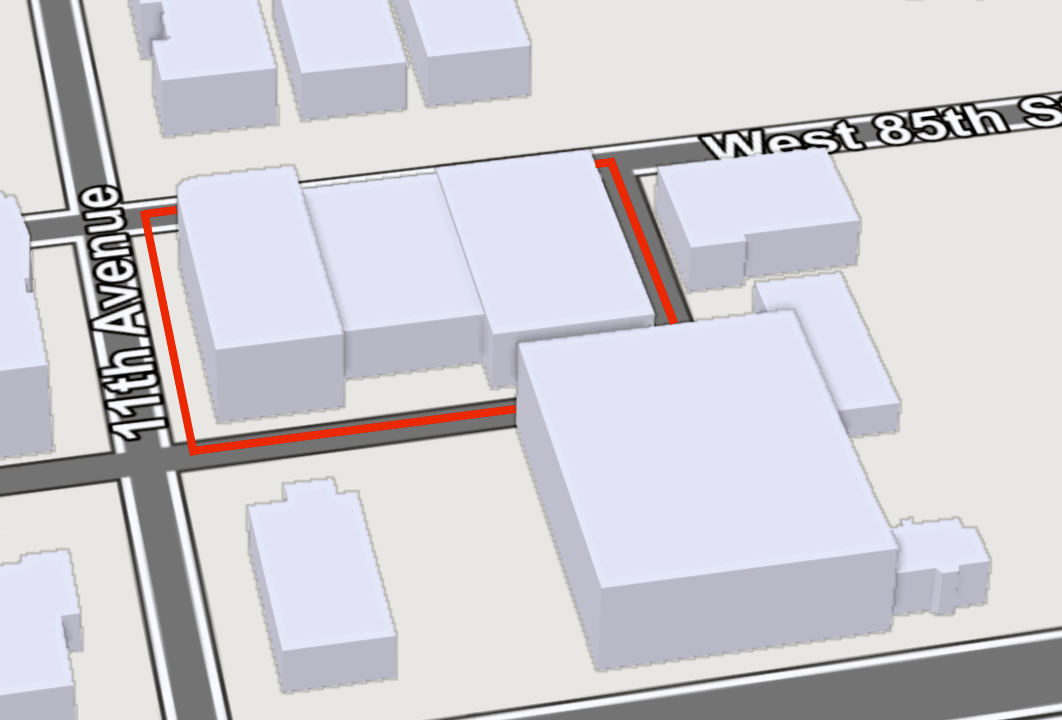
\includegraphics[width=.49\textwidth]{propagazione-osm-3d.png}
		\hfill
	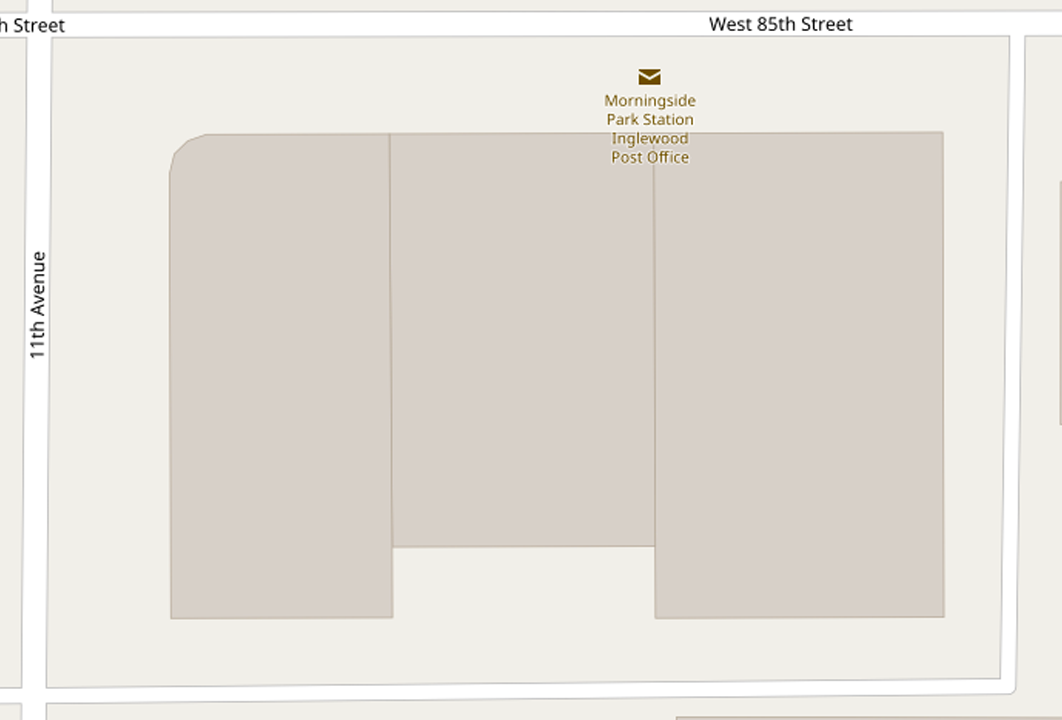
\includegraphics[width=.49\textwidth]{propagazione-osm.png}
\caption{Rappresentazione in $2$D e $3$D degli edifici utilizzati per l'esempio.\label{fig:propagazione-osm}}
\end{figure}
%
\begin{figure}[htbp]
	\centering
	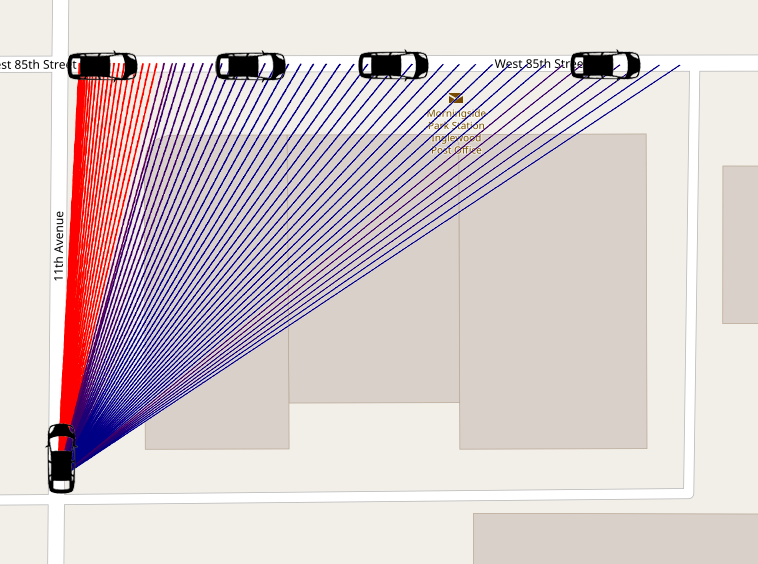
\includegraphics[width=.49\textwidth]{propagazione-2d.png}
	\hfill
	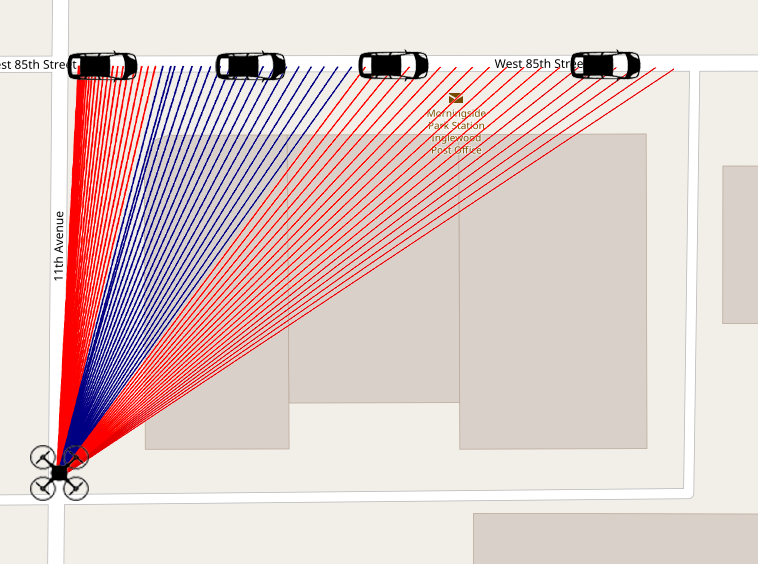
\includegraphics[width=.49\textwidth]{propagazione-3d.png}
\caption{Degradazione del valore RSS mentre il secondo veicolo è in movimento.
Ogni linea indica una trasmissione, mentre il colore rappresenta l'RSS.\label{fig:propagazione-2d-3d}}
\end{figure}
%
